\section{Industrie 4.0}
%
\subsection{Allgemein}

Industrie 4.0 ist ein Schlagwort, das die vierte industrielle 
Revolution beschreibt. Durch die Vernetzung der Maschine mit 
den Produkten wurde die traditionelle Produktionshierarchie abgebaut. 
Dezentrale Selbstorganisation ersetzt die zentrale Steuerung. 
Die Produkte werden aktiv in den Produktionsprozess eingebunden. 
Ressourcen- und Energieeinsparung ist eine Voraussetzung 
f"ur die Prozessplanung und erfolgreiche Produktion.
 Es werden so genannte intelligente Fabriken aufgebaut.
Der Name wurde zum ersten Mal auf der Hannover Messe 2011 verwendet[9]. 
In Deutschland sind die Empfehlungen zur Umsetzung des Arbeitskreises 
Industrie 4.0 an die Bundesregierung weitergeleitet worden.
 Auf der Hannover Messe 2013 wurde ein Endbericht der Arbeitsgruppe
  eingereicht und parallel dazu nahm die von den drei Fachverb"anden 
  Bitkom, VDMA und ZVEI gegr"undete Industrieplattform 4.0 
  ihre Arbeit auf. Ziel ist es, die Aktivit"aten 
  in diesem Feld in Zukunft zu koordinieren[10].
Mechatronische Systeme,Cyberphysikalische Systeme und das "Internet der 
Dinge" oder "Internet der Dienste" sind technologische 
Voraussetzungen[11]. 





\subsection{Voraussetzung der Technik}
%
\subsubsection{Mechatronische Systeme}
Mechatronische Systeme bestehen aus einem Basissystem.
Sensoren, Aktoren und ein Informationssystem.
Transformation. Die Umsetzung der
das mechatronische System, in dem es betrieben wird.
Das Basissystem ist in der Regel ein
mechanisch, elektromechanisch, hydraulisch oder pneumatisch.
Generell ist jedoch jedes physikalische System als Basissystem denkbar, 
d.h. mechatronische Systeme mit einer bestimmten 
hierarchischen Struktur k"onnen abgebildet werden[12].
Die Abbildung~\ref{fig:me} zeigt ein Beispiel eines 
mechatronischen System.

\begin{figure}[!htb]
\begin{center}
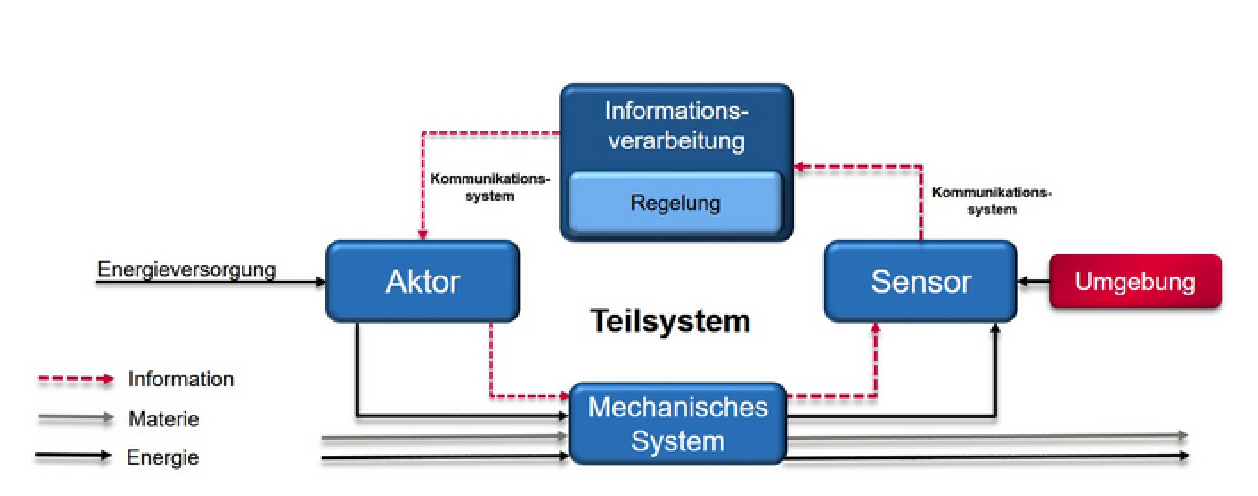
\includegraphics[height=5cm]{bilder/me.eps}
\end{center}
\caption{Mechatroniches System[12]}\label{fig:me}
\end{figure}



\subsubsection{Die Bedeutung Cyper Physical Systems}

 CPS sind mechanische Komponenten 
durch intelligente Netzwerke und Informationstechnologien miteinander verkn"upft.
 Sie erlauben die Steuerung und "uberwachung komplexer Systeme und Infrastrukturen.
 Cyber-physikalische Systeme spielen in Industrie 4.0 eine wichtige Rolle.
 Sie sind moderne mechanische Komponenten, 
 Software und Informationstechnologie. Die Vernetzung der verschiedenen 
 Komponenten "uber Netzwerke wie das Internet erm"oglicht die Steuerung, 
 Regelung und "uberwachung komplexer Infrastrukturen. 
 Der Informationsaustausch zwischen Objekten und vernetzten 
 Systemen kann in Echtzeit, drahtlos oder drahtgebunden erfolgen. 
 Die Komponenten cyber-physikalischer Systeme umfassen sowohl
  mobile Ger"ate als auch station"are Maschinen, Systeme und Roboter. 
  Cyber-physikalische Systeme spielen in Industrie 4.0 eine wichtige 
  Rolle. Die technologischen Grundlagen des CPS werden durch 
  Naturwissenschaften wie Informatik, Mathematik, Maschinenbau, 
  Elektrotechnik und Robotik geliefert[13].\newline
  Das Betriebsprinzip ist auf vernetzte Sensoren, 
  Aktoren und Software aufgebaut. 
  Sensoren ermitteln Messdaten aus der physikalischen Welt 
  und "ubertragen sie "uber Netzwerke an die Software, die sie verarbeitet. 
  Daraus resultieren die Regeldaten, die die Software "uber 
  das Netzwerk an die Stellglieder "ubermittelt. 
  Cyberphysikalische Systeme sind in Abbildung~\ref{fig:cps} aufgebaut 
  und zeichnen sich durch einen hohen Grad 
  an Komplexit"at aus und werden beispielsweise f"ur den Aufbau von Smart Power Grids, 
  modernen Produktionsanlagen oder in der Medizintechnik eingesetzt.
  Viele verschiedene Komponenten und Technologien werden ben"otigt, 
  damit cyberphysikalische Systeme ihre Aufgaben erfüllen können.
   Dazu gehören Zum Beispiel:
 \begin{itemize}
   \item Sensoren
    \item Aktoren 
     \item eingebettete Systeme
      \item Netzwerkinfrastrukturen [14]
    \end{itemize}
   
  
  
  
 %





    
    
 \subsubsection{Erkl"arung des Begriffs Das Internet der Dinge}
 
 Der Begriff Internet der Dinge wie gezeigt in Abbildung~\ref{fig:F} erkl"art,
  dass der Computer zunehmend wie
   ein Ger"at verloren geht und durch intelligente Objekte 
   zu ersetzen ist.Um im Interesse der Menschen zu sein, 
   sollte das Internet der Dinge die Menschen bei 
   ihren Aktivit"aten unbemerkt st"arken. 
   Kleinere eingebetteten Computer sind so konstruiert, 
   dass sie Menschen helfen, ohne abzulenken oder Aufmerksamkeit zu ablenken. 
   
  Das Internet der Dinge beschreibt die Verbindung von klar 
   identifizierbaren physischen Objekten mit einer virtuellen 
   Darstellung in einer internetgleichen Struktur. 
   Sie besteht nicht mehr nur aus menschlichen Beteiligten, 
   sondern auch aus Dingen[15].
 
 
 \begin{figure}[!htb]
\begin{center}
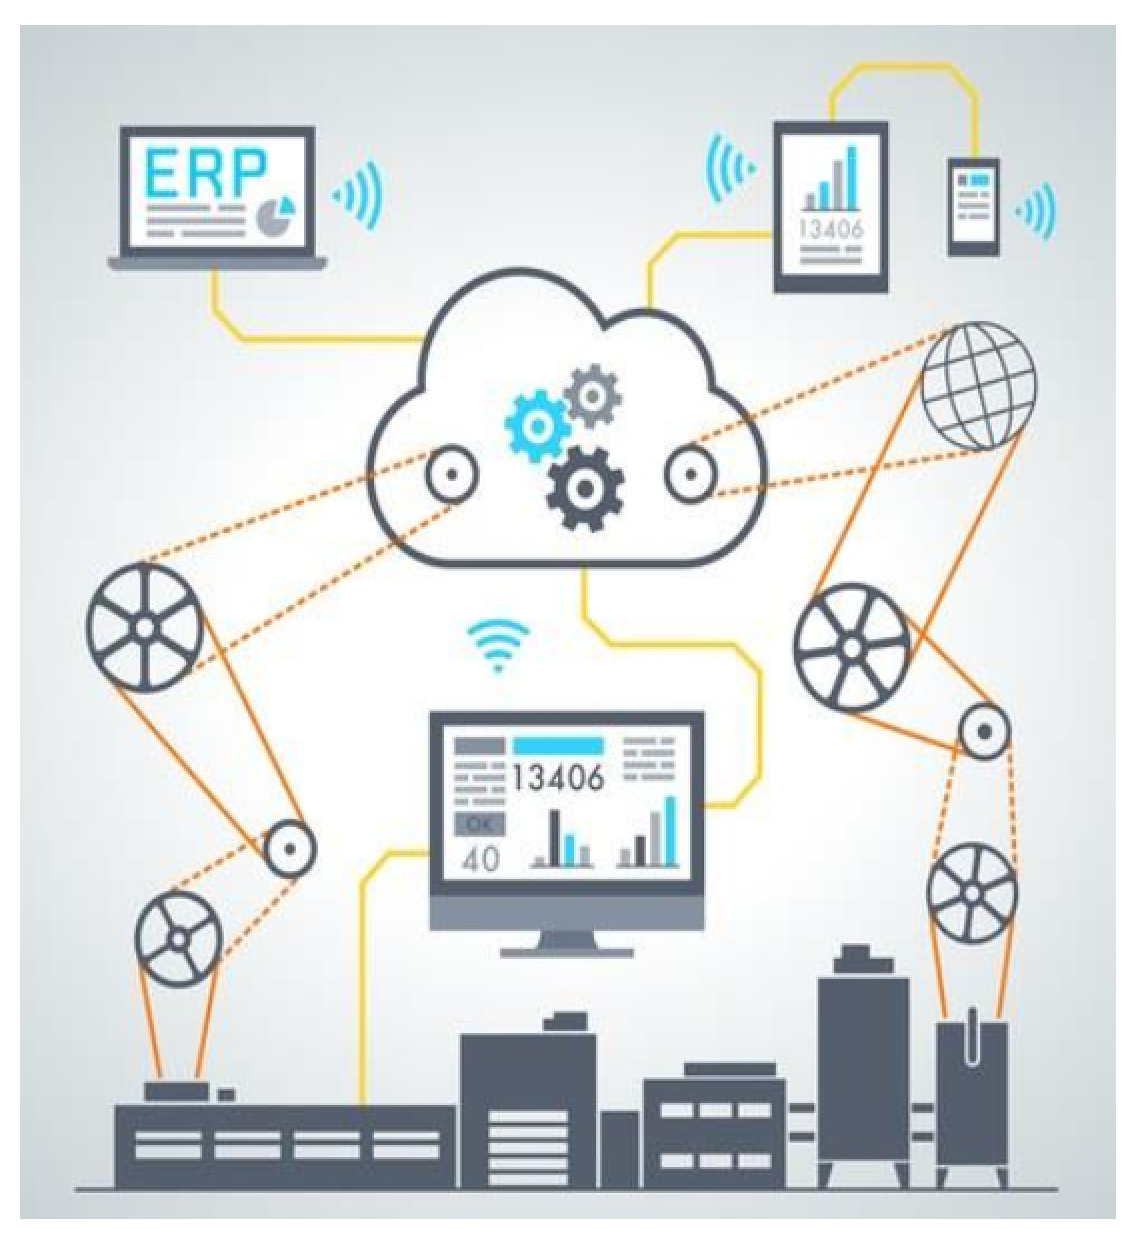
\includegraphics[height=8cm]{bilder/F.eps}
\end{center}
\caption{Internet der Dinge[16]}\label{fig:F}
\end{figure}

Die automatische Identifikation durch RFID wird oft als Basis 
f"ur das Internet der Dinge betrachtet. 
Objekte k"onnen aber auch mittels Barcode oder 
2D-Code eindeutig identifiziert werden. 
Ger"ate wie Sensoren und Aktoren erm"oglichen
 die Erweiterung der Funktionalit"at, 
 indem sie Zust"ande erfassen oder Aktionen durchf"uhren.
  Das Internet der Dinge erm"oglicht es, 
  reale Informationen effektiv zu erfassen und digital 
  zu verarbeiten, unter den technischen Bedingungen und Anforderungen, 
  die oft als notwendig betrachtet werden, 
  um die Medienl"ucke zwischen der realen und 
  der virtuellen Welt zu reduzieren. 
  Die Internetsichten der Objekte werden 
  in die Produktionsumgebung "ubertragen. 
  Die Industrie wird in der Lage sein, 
  sehr stark individualisierte Produkte in kleinen Mengen 
  (bis zu einer einzigen Menge) herzustellen, 
  und zwar bei hoher Ressourcenproduktivit"at 
  und entsprechender Geschwindigkeit[17].







 


